\documentclass[tikz,border=10pt]{standalone}
% Scale: s = 0.021448 cm/px, origin at circle centre O
\begin{document}
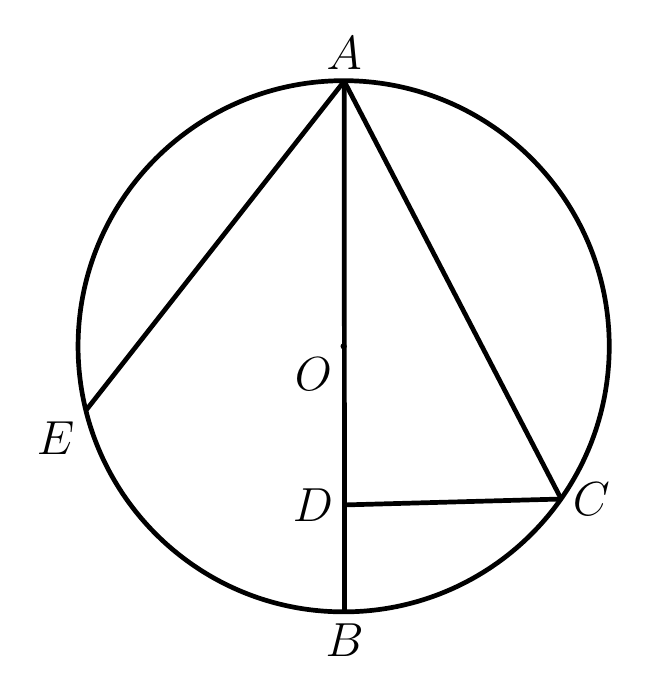
\begin{tikzpicture}[line width=1.7pt, line join=round, font=\fontsize{18}{21.6}\selectfont]
  % Points (cm), y flipped from image pixels
  \coordinate (O) at (0,0);
  \coordinate (A) at (0.007,3.367);
  \coordinate (B) at (0.011,-3.373);
  \coordinate (E) at (-3.273,-0.815);
  \coordinate (C) at (2.763,-1.940);
  \coordinate (D) at (0.011,-2.015);

  % Circle, radius 157.27 px
  \draw (O) circle[radius=3.373];

  % Segments: AB, AE, AC, DC
  \draw (A) -- (B);
  \draw (A) -- (E);
  \draw (A) -- (C);
  \draw (D) -- (C);

  % Centre dot
  \fill (O) circle[radius=0.04];

  % Labels
  \node[above] at (A) {$A$};
  \node[below left] at (O) {$O$};
  \node[below left] at (E) {$E$};
  \node[right] at (C) {$C$};
  \node[left] at (D) {$D$};
  \node[below] at (B) {$B$};
\end{tikzpicture}
\end{document}